\documentclass{article}
\usepackage[utf8]{inputenc}
\usepackage[english,vietnamese]{babel}
\usepackage{graphicx} % Required for inserting images
\usepackage{float} % Allows better image placement
\usepackage{titling} % Allows control over title placement
\usepackage{hyperref}  % Required for clickable links
\usepackage{amsmath}
\usepackage{listings}
\usepackage{enumitem}
\usepackage{tikz}
\usetikzlibrary{shapes.geometric, arrows}
\tikzstyle{startstop} = [rectangle, rounded corners, minimum width=3cm, minimum height=1cm,text centered, draw=black, fill=purple!30]
\tikzstyle{process} = [rectangle, minimum width=3cm, minimum height=1cm, text centered, draw=black, fill=green!30]
\tikzstyle{ellipse} = [circle, minimum width=3cm, minimum height=1cm, text centered, draw=black, fill=blue!30]

\tikzstyle{arrow} = [thick,->,>=stealth]

\hypersetup{
    colorlinks=true,   % Enable colored links
    linkcolor=black,    % Color of internal links (sections, TOC, etc.)
    urlcolor=blue      % Color for URLs
}

\title{Report Labwork}
\author{
    Vu Trong Bach - 22BI13056\\  
}
\date{November 2024}

\setlength{\droptitle}{-5em} % Adjust the vertical space before the title

\begin{document}

\begin{figure}[H]
    \textsc{\large \bfseries University of Science and Technology of Ha Noi}\\[0.5cm]
    \centering
    
\includegraphics[width=0.8\linewidth]{usth.png}
    \label{fig:project-overview}

    \vspace{1cm}
 
    \textsc{\large \bfseries Practical Labwork 1}\\[1cm]

    \textsc{\Large \bfseries Distributed System - Le Nhu Chu Hiep}\\[1cm]
\end{figure}


% Manual title to avoid page break
\vspace{1cm}
\begin{center}
    \huge \textbf{\thetitle} \\[0.5cm]
    \Large \theauthor [0.5cm]
    \large \thedate
\end{center}

\vspace{4cm}
\tableofcontents

\newpage
\section{Introduction}
The practical work aimed to implementation a 1-to-1 file transfer using TCP/IP via sockets. This will help us understand how data communication works at the transport layer using the TCP protocol.

\subsection{TCP and File Transfer over Sockets}
TCP-Transmission Control Protocol-guarantees reliable, ordered, and error-checked delivery of data. File transfer over sockets involves the following:
\begin{itemize}
    \item Establish a connection between the client and the server.
    \item Data transfer from one machine to another.
    \item Properly handling connection closure and EOF (End of File).
\end{itemize}

\section{Protocol Design}
\subsection{Client-Server Interaction Diagram}
Below is the interaction diagram showing how the client and server communicate:

\begin{figure}[h]
    \centering
    \begin{tikzpicture}[node distance=2cm]

    % Nodes
    \node (start) [startstop] {Server: Start};
    \node (bind) [process, below of=start] {Bind and Listen};
    \node (accept) [process, below of=bind] {Accept Connection};
    \node (read) [process, below of=accept] {Received File in Chunks};
    \node (close) [startstop, below of=read] {Close Connection};

    % Arrows for Server
    \draw [arrow] (start) -- (bind);
    \draw [arrow] (bind) -- (accept);
    \draw [arrow] (accept) -- (read);
    \draw [arrow] (read) -- (close);

    % Client side
    \node (start_client) [startstop, right of=start, xshift=6cm] {Client: Start};
    \node (connect) [process, below of=start_client] {Attemp to connect to server};
    \node (request) [process, below of=connect] {Successfully connected};
    \node (receive) [process, below of=request] {Upload File};
    \node (close_client) [startstop, below of=receive] {Close Connection};

    % Arrows for Client
    \draw [arrow] (start_client) -- (connect);
    \draw [arrow] (connect) -- (request);
    \draw [arrow] (request) -- (receive);
    \draw [arrow] (receive) -- (close_client);

    % Connection Arrows
    \draw [arrow] (accept.east) -- ++(0.5,0) |- (request.west);
    \draw [arrow] (receive.west) -- ++(0.5,0) |- (read.east);

    \end{tikzpicture}
    \caption{Client-Server Interaction for TCP File Transfer}
    \label{fig:protocol}
\end{figure}

\subsection{Logic of the Protocol}
\begin{enumerate}
    \item The server sets up by binding to an IP address and port, then waits for connections from clients.
    \item The client starts the process by connecting to the server.
    \item Once connected, the client asks for a file. After we typing in the file that we want to transfer, the program will automatically transfer the file to the server.
    \item Once the server received the file, it will store the file in a folder.
    \item After successfully transfer, both the client and server will close the connection.
\end{enumerate}

\section{System Organization}
\subsection{System Architecture}
The system consists of two main components: the client and the server. Their roles are described in the following:
\begin{itemize}
    \item \textbf{Server:} Handles incoming connections and sends requested files to clients.
    \item \textbf{Client:} Connects to the server and upload files.
\end{itemize}

\subsection{Architecture Diagram}
\begin{figure}[h]
    \centering
    \begin{tikzpicture}[node distance=2cm]

    % Nodes
    \node (server) [ellipse] {Server};
    \node (network) [ellipse, right of=client, xshift=4cm] {Network};
    \node (client) [ellipse, right of=network, xshift=4cm] {Client};

    % Arrows
    \draw [arrow] (server.east) -- node[anchor=south] {Open Connection} (network.west);
    \draw [arrow] (network.east) -- node[anchor=south] {Forward to Client} (server.west);
    \draw [arrow] (server.west) -- node[anchor=north] {Send Data} (network.east);
    \draw [arrow] (network.west) -- node[anchor=north] {Received data from Client} (client.east);

    \end{tikzpicture}
    \caption{System Architecture for TCP File Transfer}
    \label{fig:system}
\end{figure}

\section{Implementation}
\subsection{Key Code Snippets}
\subsubsection{Server Code}
The server code is responsible for listening to connections and sending files:
\begin{lstlisting}[language=Python, caption=Server Code]
# server.py
import socket
import os

# Server configuration
HOST = '172.27.242.41'  # Replace with your server's IP address
PORT = 8386  # Port for communication
SAVE_DIR = "uploaded_files"  # Directory to save received files

def start_server():
    # Ensure the save directory exists
    if not os.path.exists(SAVE_DIR):
        os.makedirs(SAVE_DIR)

    # Create a TCP socket
    server_socket = socket.socket(socket.AF_INET, socket.SOCK_STREAM)
    server_socket.bind((HOST, PORT))  # Bind to the server IP and port
    server_socket.listen(1)  # Allow one client connection at a time
    print(f"Server listening on {HOST}:{PORT}...")

    while True:
        # Accept a connection from a client
        conn, addr = server_socket.accept()
        print(f"Connection established with {addr}")

        try:
            # Receive the filename first, up to the newline character
            filename = b""
            while True:
                byte = conn.recv(1)
                if byte == b'\n':  # Delimiter indicates the end of the filename
                    break
                filename += byte
            filename = filename.decode('utf-8')  # Decode bytes to string
            print(f"Receiving file: {filename}")

            # Define full path to save the file
            save_path = os.path.join(SAVE_DIR, filename)

            # Open the file to save the incoming data
            with open(save_path, 'wb') as file:
                while True:
                    data = conn.recv(1024)  # Receive file data in chunks (1KB)
                    if not data:  # Condition to check if the file transfer is complete
                        break
                    file.write(data)

            print(f"File '{filename}' received and saved in '{SAVE_DIR}/'.")
        except Exception as e:
            print(f"Error receiving file: {e}")
        finally:
            conn.close()  # Close the client connection
            print(f"Connection with {addr} closed.")

if __name__ == "__main__":
    start_server()

\end{lstlisting}

\subsubsection{Client Code}
The client code connects to the server and receives the file:
\begin{lstlisting}[language=Python, caption=Client Code]
# client.py
import socket
import os

# Server configuration
SERVER_IP = input("Enter the server's IP address: ")  # Enter Server's IP address
PORT = 8386  # Server's port

def send_file():
    try:
        # Create a TCP socket
        client_socket = socket.socket(socket.AF_INET, socket.SOCK_STREAM)
        print(f"Attempting to connect to {SERVER_IP}:{PORT}...")
        client_socket.connect((SERVER_IP, PORT))
        print(f"Connected to server at {SERVER_IP}:{PORT}")

        # Get the filename and ensure it exists
        while True:
            filename = input("Enter the full file name (with extension): ")
            if os.path.isfile(filename):  # Ensure the file exists
                break
            print("File not found. Please try again.")

        # Extract just the file name for sending (without the directory path)
        base_filename = os.path.basename(filename)

        # Send the filename to the server
        client_socket.send(base_filename.encode('utf-8') + b'\n')  # Send filename with newline delimiter

        # Open the file and send its content in chunks
        with open(filename, 'rb') as file:
            print(f"Sending file '{base_filename}' to the server...")
            while chunk := file.read(1024):  # Read in chunks of 1KB
                client_socket.send(chunk)

        print(f"File '{base_filename}' sent successfully to the server.")
        client_socket.close()

    except ConnectionRefusedError:
        print("Connection failed: Ensure the server is running and reachable.")
    except socket.timeout:
        print("Connection timed out: Server is taking too long to respond.")
    except Exception as e:
        print(f"An unexpected error occurred: {e}")

if __name__ == "__main__":
    send_file()

\end{lstlisting}

\section{Responsibility Distribution}
The project tasks were distributed among the members of the group as follows:
\begin{itemize}
    \item \textbf{Huy:} Run the client file to connect to my server.
    \item \textbf{Bach(me):} Send file "test" from server to client.
    \item \textbf{Bach(also me):} Designed the protocol and documented the report.
\end{itemize}

\begin{figure}[h!]
    \centering
    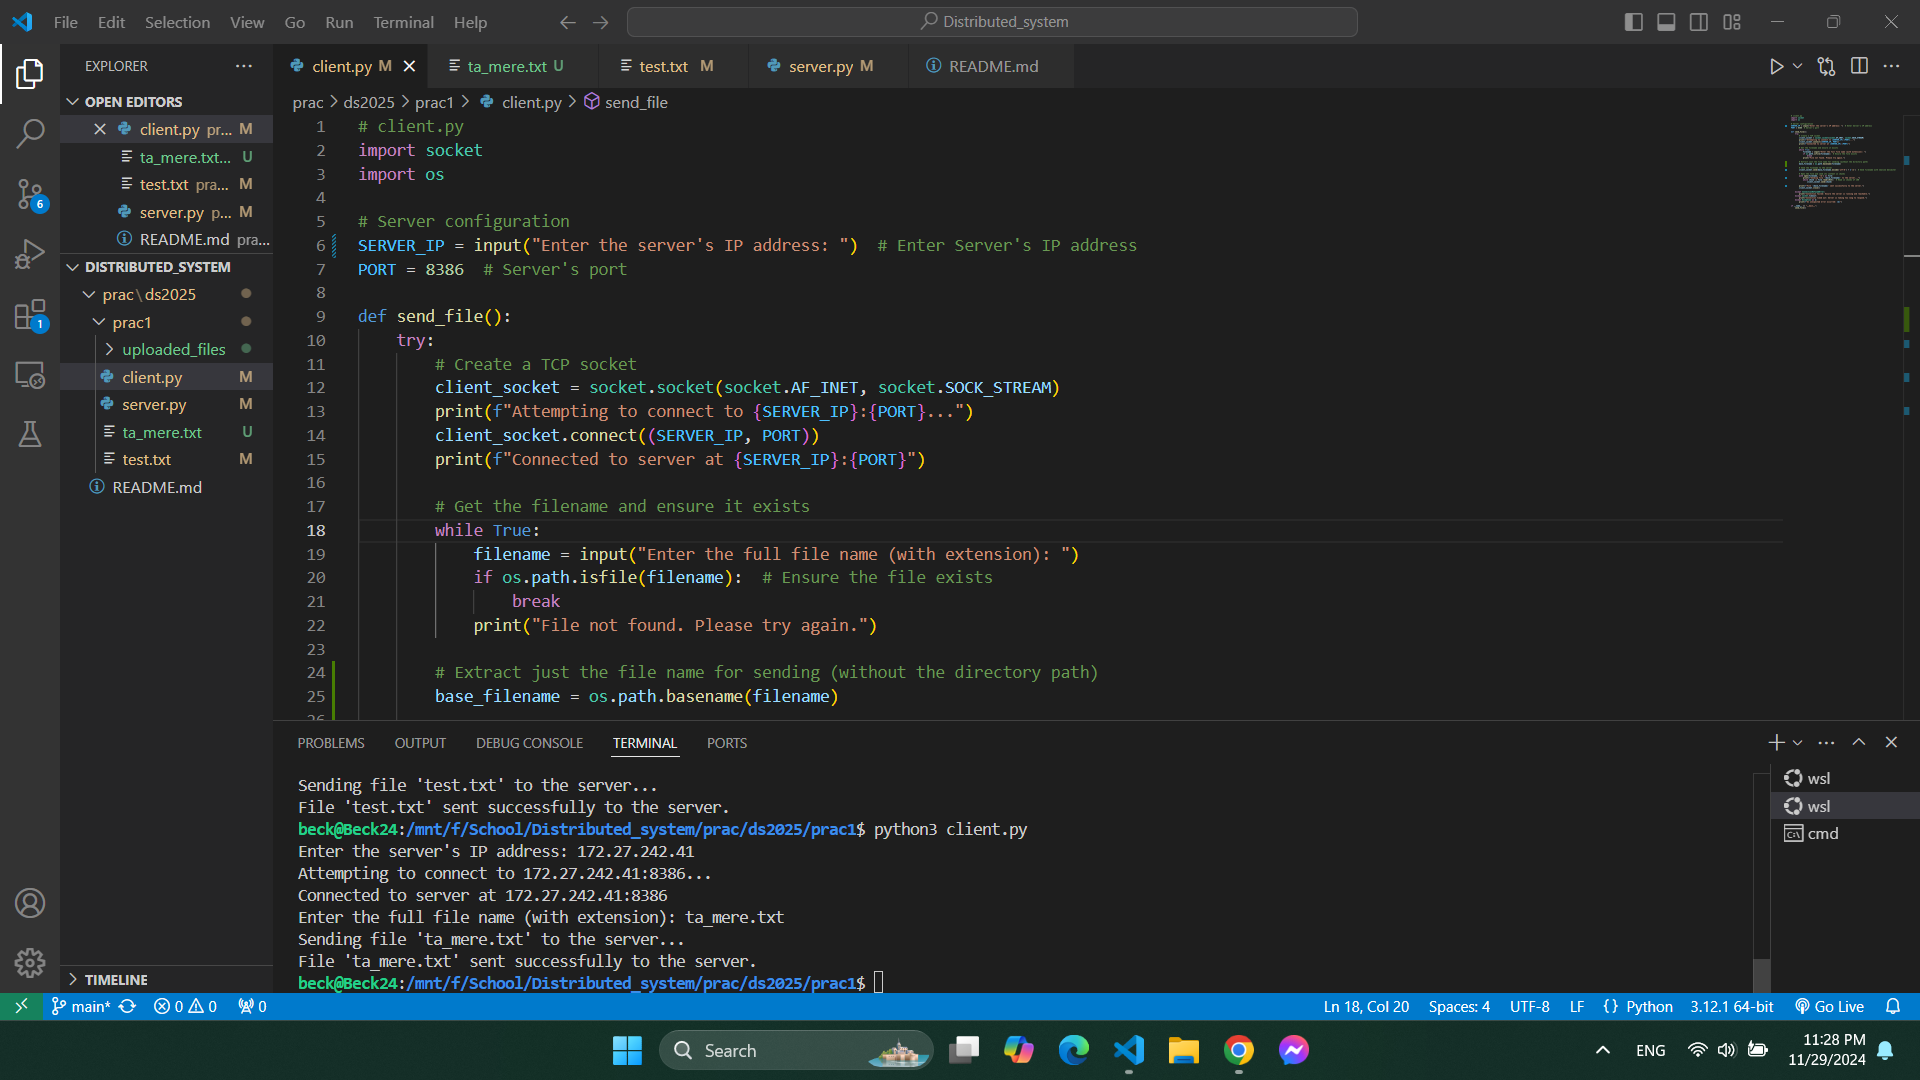
\includegraphics[width=0.8\textwidth]{Connection_client.png} % Thay thế bằng đường dẫn ảnh của bạn
    \caption{Client connects to server and sends file}
    \label{fig:client}
\end{figure}
\clearpage
\begin{figure}[h!]
    \centering
    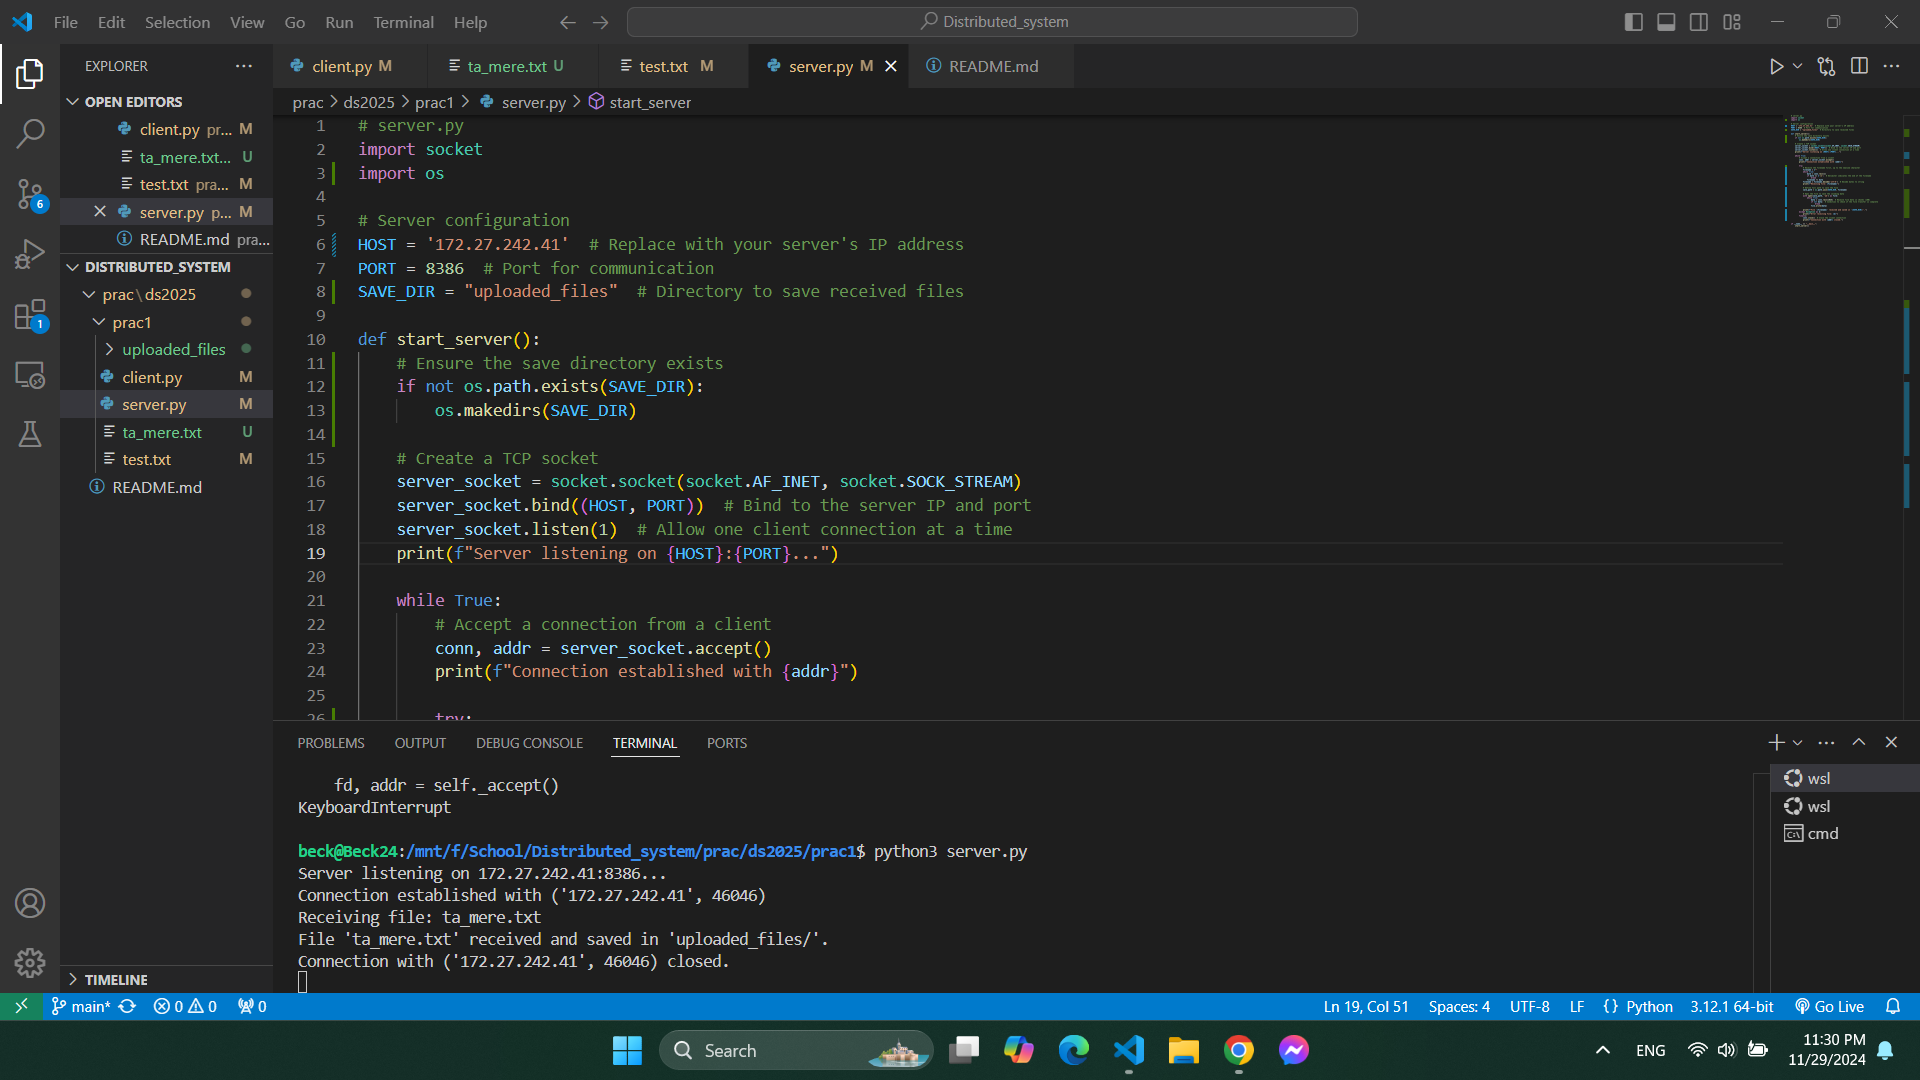
\includegraphics[width=0.8\textwidth]{Connection_server.png} % Thay thế bằng đường dẫn ảnh của bạn
    \caption{Server connects to client and receives file}
    \label{fig:server}
\end{figure}

\section{Conclusion}
This labwork offered practical insights into TCP/IP and socket programming, demonstrating how file transfer can be implemented in a client-server architecture. During the implementation, challenges such as managing EOF signals and handling connection errors were encountered and effectively addressed using robust exception handling and thorough testing. Future enhancements could include implementing encryption to ensure secure file transfers and extending the system to handle multiple clients simultaneously, improving scalability and security.

\end{document}